\documentclass[12pt]{book}
\usepackage{diffyqssetupUB}

\begin{document}



%extra material {Nonhomogeneous equations}

\subsection{Undetermined coefficients with Python}

If you'd like to check your answer to an undetermined {\color{red}coefficient} 
{\color{blue}coefficients} problem, 
you can do it using sympy, as we show below for the differential equation $\frac{d^2y}{dx^2} + 2 \frac{dy}{dx} + 2 y = \cos 2x$
and the guess $y = A\cos 2x + B \sin 2x$.
{\color{teal}BH c2 as shorthand for cos(2*x) is too easily confused with c2 as a constant. 
Suggest use cos2x, sin2x. JR Suggested changes made.
}
\begin{small}
\begin{verbatim}
from resources306 import *
x,A,B = sp.symbols('x A B')
cos2x,sin2x = sp.cos(2*x),sp.sin(2*x)    # shorthand
y = A*cos2x + B*sin2x  # our guessed form of the solution
de_lhs = sp.diff(y,x,x) + 2*sp.diff(y,x) + 2*y
de_rhs = cos2x
de = de_lhs - de_rhs # shove everything to the LHS, equate this to 0
de
\end{verbatim}
\end{small}
$$ - 4 A \sin{\left (2 x \right )} + 2 A \cos{\left (2 x \right )} + 2 B \sin{\left (2 x \right )} + 4 B \cos{\left (2 x \right )} - 4 \left(A \cos{\left (2 x \right )} + B \sin{\left (2 x \right )}\right) - \cos{\left (2 x \right )} $$
\begin{small}
\begin{verbatim}
eqs = [ de.coeff(cos2x), de.coeff(sin2x)) ]
eqs
\end{verbatim}
\end{small}
$$\left [ 2 A + 4 B - 1, \quad - 4 A + 2 B\right ]$$
\begin{small}
\begin{verbatim}
sp.solve( eqs, [A,B] )
\end{verbatim}
\end{small}

$$ \left \{ A : \frac{1}{10}, \quad B : \frac{1}{5}\right \} $$



%extra material {Forced oscillations and resonance}


\subsection{Symbolic computation with Python}

As an example of symbolic computation in Python, 
we repeat the above computation using sympy.

\begin{small}
\begin{verbatim}
from resources306 import *
a,b,w,w0,p,t,G0  = sp.symbols('a b w w0 p t G0')
x = a*sp.cos(w*t) + b*sp.sin(w*t)
# Write the DE with everything on the LHS, implicitly set to 0
de = sp.diff(x,t,t) + 2*p*sp.diff(x,t) + w0**2*x -  G0*sp.cos(w*t)  
display(de)
dec = de.subs(t,0)         # get the coefficient of cos(wt)
des = de.subs(t,sp.pi/2/w) # get the coefficient of sin(wt)
display(dec); display(des)
sol = sp.solve([dec,des],[a,b])
display(sol)
amp = sp.simplify( sp.sqrt(a**2 + b**2).subs(sol) )
display( amp )
amp = amp.subs({G0:1,w0:1})  # choose units of time and amplitude
for pval in [2,1,0.5,0.25,0.125,0.0625]:
        ampp = amp.subs(p,pval)
        expressionplot( ampp, w, 0, 3, label='damping = '+str(pval) )
plt.legend()
plt.xlabel('forcing frequency, w'); plt.ylabel('amplitude of response')
plt.savefig('myresonanceplot.png')
\end{verbatim}
\end{small}

%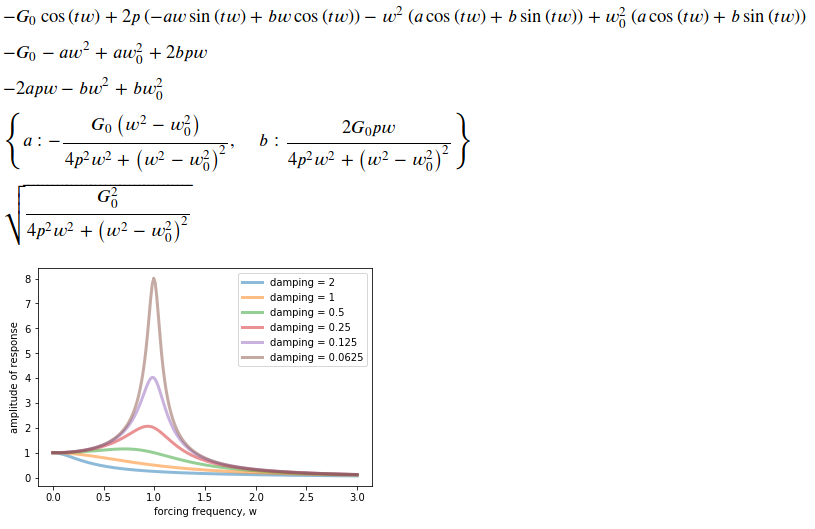
\includegraphics[width=6.5in]{additional_figures/forcing_and_resonance_output.png}
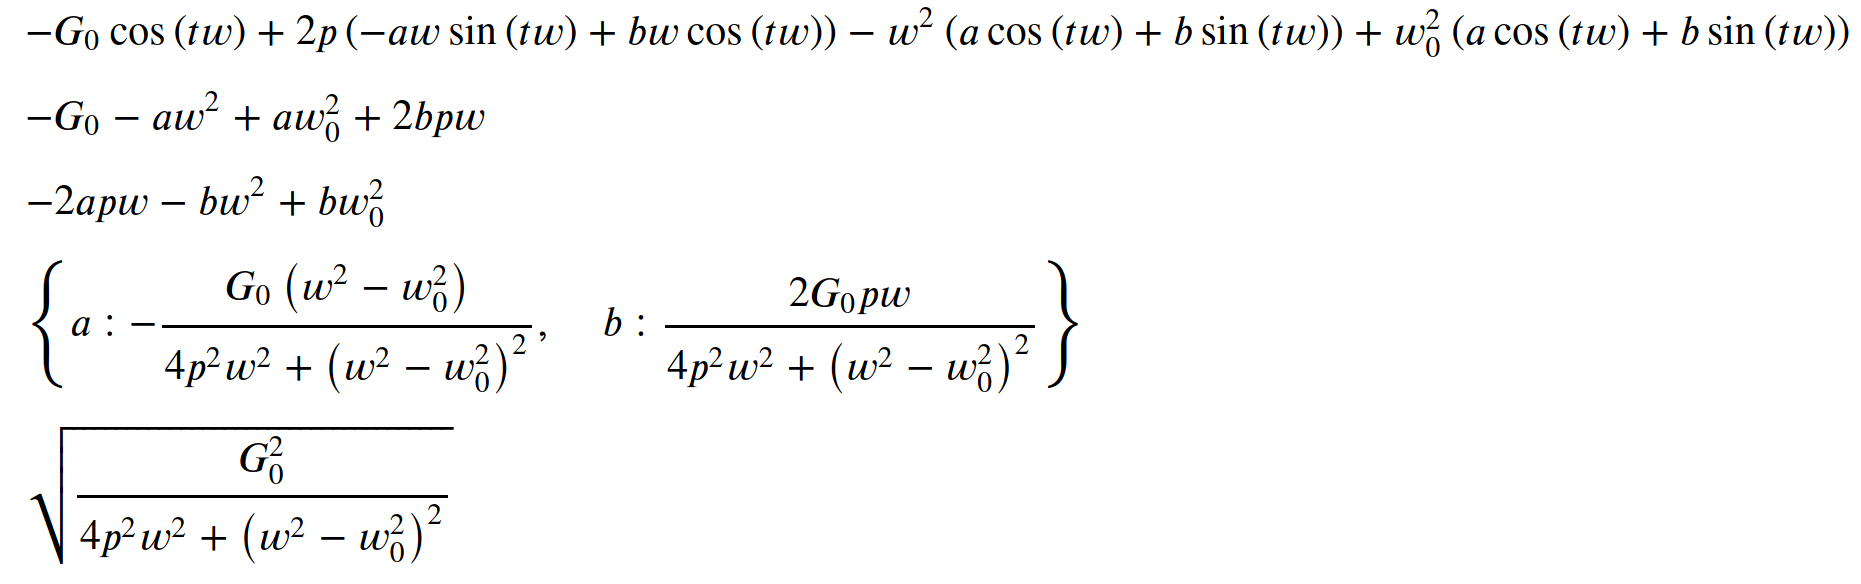
\includegraphics[width=6.5in]{additional_figures/forcing_and_resonance_symbols.png}
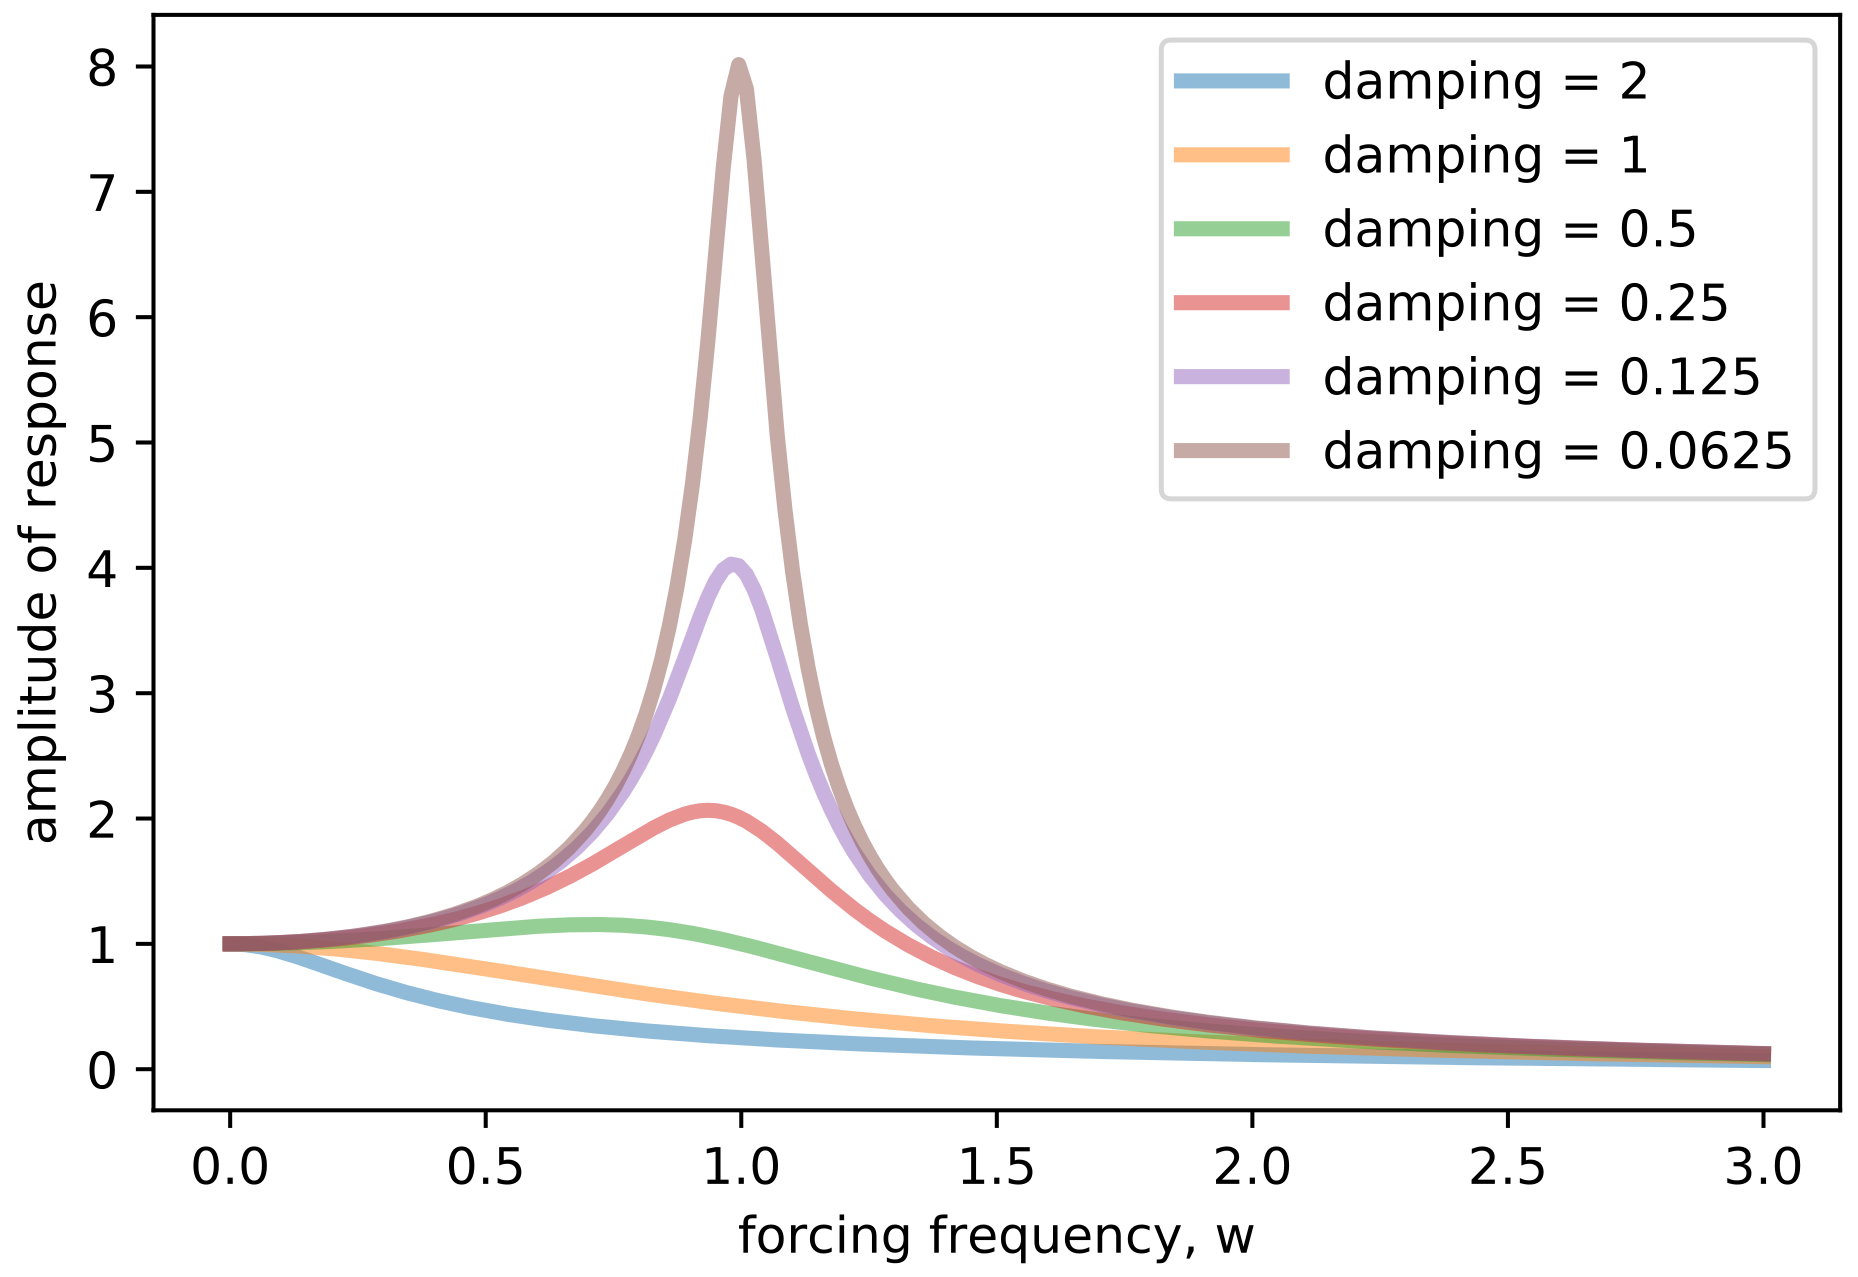
\includegraphics[width=4.5in]{additional_figures/forcing_and_resonance_plot.png}

{\color{teal}BH Missing figure. JR I guess this was before I uploaded all the figures.}
\end{document}

